\documentclass[tikz]{standalone}
\usepackage{tikz}
\usepackage[AutoFakeBold=true,AutoFakeSlant=true]{xeCJK}
\usepackage[zihao=-4,UTF8,heading=true]{ctex}
\usepackage[simplified]{pgf-umlcd}
\usetikzlibrary{fit} %形状
\usetikzlibrary{positioning} %不加方向运算可能出错
\usetikzlibrary{arrows.meta} %箭头
\usetikzlibrary{calc}

\setCJKmainfont{微软雅黑}
\begin{document}
	\thispagestyle{empty}
    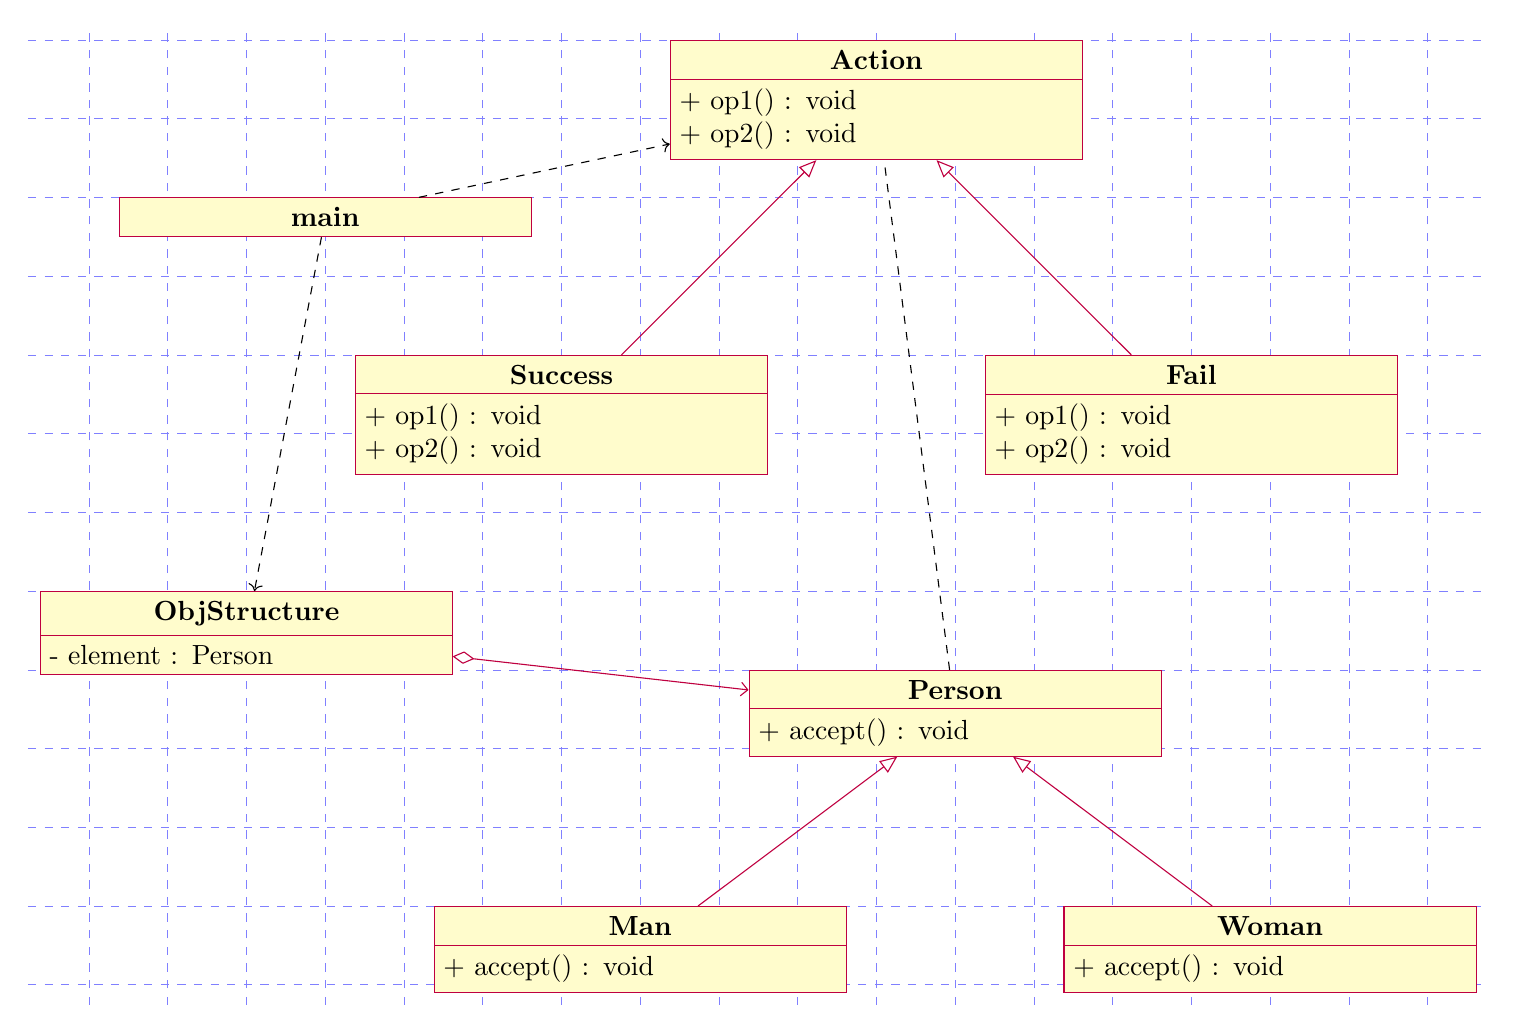
\begin{tikzpicture}[show background grid]
        \begin{class}[text width=5cm]{Action}{0,0}
            \operation{+ op1() : void}
            \operation{+ op2() : void}
        \end{class}
        \begin{class}[]{Success}{-4,-4}
            \inherit{Action}
            \operation{+ op1() : void}
            \operation{+ op2() : void}
        \end{class}
        \begin{class}[]{Fail}{4,-4}
            \inherit{Action}
            \operation{+ op1() : void}
            \operation{+ op2() : void}
        \end{class}
        \begin{class}[]{ObjStructure}{-8,-7}
            \attribute{- element : Person }
        \end{class}
        
        \begin{class}[]{Person}{1,-8}
            \operation{+ accept() : void}
        \end{class}
        \begin{class}[]{Man}{-3,-11}
            \inherit{Person}
            \operation{+ accept() : void}
        \end{class}
        \begin{class}[]{Woman}{5,-11}
            \inherit{Person}
            \operation{+ accept() : void}
        \end{class}
        \draw [dashed] (Person) -- (Action);

        \aggregation{ObjStructure}{}{}{Person}
        \begin{class}[]{main}{-7,-2}
        
        \end{class}
        \draw [dashed, ->] (main) -- (Action);
        \draw [dashed, ->] (main) -- (ObjStructure);
    \end{tikzpicture}

\end{document}